% !TeX encoding = UTF-8
% !TeX root = choix_extensions.tex
\chapter{Bibliographies et index}





\section{Workflow}

Il y a trois étapes pour faire une bibliographie avec \LaTeX. Il existe d'innombrables manières de le faire, des plus manuelles jusqu'aux plus automatisées comme celle choisie ici.
\begin{enumerate}
	\item Créer une base bibliographique
		\begin{itemize}
			\item A faire : récolter les informations pour chaque ouvrage à citer et les mettre correctement en forme dans un fichier \incmd{.bib}.
			\item Moyen : Zotero et son add-on BetterBibTeX. \\
				Zotero est un logiciel spécialisé dans la gestion des références bibliographiques. Il est mondialement utilisé dans les universités et les hautes écoles.
		\end{itemize} 
	\item Citer les ouvrages voulus
		\begin{itemize}
			\item A faire : utiliser les diverses commandes pour citer une référence, une partie de référence (p. ex. uniquement l'auteur).
			\item Moyen : glisser-déposer des références depuis Zotero et utiliser les aides à la saisie de TeXstudio.
		\end{itemize}
	\item Générer la bibliographie
		\begin{itemize}
			\item A faire : configurer les styles et les options, choisir l'emplacement de la bibliographie, et générer la bibliographie.
			\item Moyen : le compilateur biber et la librairie biblatex.
		\end{itemize}
\end{enumerate}

L'installation de Zotero et les configurations requises sont détaillées dans la section \ref{sec:installationConfigurationBibliographie} ci-dessous.





\section{Création de la base bibliographique}


\subsection{Pour des références mentionnées sur Internet}
\label{sec:referenceSurInternet}

C'est le but de Zotero (voir \ref{sec:installationConfigurationBibliographie}) :
\begin{enumerate}
	\item référencez automatiquement les ouvrages mentionnés et les sites visités d'un simple clic dans Zotero;
	\item adaptez les entrées automatiques selon vos exigences en tapant simplement les informations dans Zotero;
	\item faites un clic droit dans l'entrée Zotero correspondante et demandez \incmd{Generate BibTeX Keys}. Cela ajoute un champ \incmd{extra} à l'entrée Zotero avec un contenu \incmd{bibtex:<clé>}. Au besoin éditer la \incmd{<clé>} pour la rendre plus explicite\dots \ Cette clé est l'identifiant de l'entrée bibliographique et sera utilisée pour citer l'entrée.
	\item avec la configuration proposée ci-dessous (voir \ref{sec:installationConfigurationBibliographie}), le fichier \incmd{.bib} se met à jour sans intervention.	
\end{enumerate}

\remarque*{
	Si le fichier \incmd{.bib} n'est pas mis à jour suffisamment rapidement, on peut la déclencher en allant dans : \newline
	\incmd{préférences de Zotero} \textrightarrow onglet \incmd{Better BibTeX} \textrightarrow \incmd{Automatic Export} \newline 
	sélectionner l'export voulu et cliquez sur le bouton \incmd{Export}.
}


\subsection{Pour des ouvrages en arbre mort}

Pour récupérer des informations bibliographiques à partir d'ouvrages papier, il existe deux options :
\begin{enumerate}
	\item retrouver cet ouvrage sur Internet et le référencer avec Zotero;
	\item créer une entrée automatique avec Zotero en lui fournissant l'ISBN du livre (icône \raisebox{-1ex}{
\includegraphics[height=3ex]{captures/zotero_doc_par_id.png}}).
\end{enumerate}





\section{Citer les ouvrages}


\subsection{Citer une référence}

Avec la configuration proposée ci-dessous (voir \ref{sec:installationConfigurationBibliographie}), il suffit de glisser-déposer un ouvrage depuis Zotero dans le code \LaTeX pour introduire un \mintinline{latex}{\autocite{clé}}.

\remarques*{
	\label{rem:citerReference}
	\listtopsep
	\begin{enumerate}
		\item En fait \inlatex{\autocite} choisit automatiquement l'une des commandes suivantes selon le style de la bibliographie :
			\begin{itemize}
				\item \inlatex{\cite} pour citer sans fioritures;
				\item \inlatex{\parencite} pour forcer l'utilisation des parenthèses;
				\item \inlatex{\footcite} pour forcer l'utilisation de note de bas de page;
				\item \inlatex{\textcite} pour éviter les parenthèses.
			\end{itemize}
		\item Ces commandes peuvent prendre deux options :
			\begin{itemize}
				\item \inlatex{\autocite[voir][p. 152]{clé}} va faire précéder la référence de "voir" et la faire suivre de ", p. 152" (avec la virgule);
				\item \inlatex{\autocite[postnote]{clé}} écrit uniquement après la référence;
				\item \inlatex{\autocite[prenote][]{code}} n'écrit qu'avant la référence. \attention aux deux crochets vides dans ce cas.
			\end{itemize}
		\item Il existe aussi des possibilités de ne citer qu'une partie de la référence, par exemple \inlatex{\citeauthor{clé}} pour ne citer que l'auteur ou \inlatex{\citeyear{clé}} pour l’année de publication. Voir la section \textit{Citation Commands} de la documentation du package \incmd{biblatex}.
	\end{enumerate}
}


\subsection{Citer un extrait}

Pour citer un extrait d'un texte, on utilise les commandes du package \incmd{csquotes} :
\begin{enumerate}
	\item Pour une citation sans référence à la source :
		\begin{itemize}
			\item \inlatex{\enquote{citation}} : pour un texte court, inclus dans le paragraphe en cours et avec des guillemets francophones.
			\item \inlatex{\blockquote{citation}} : si la citation est courte, c'est comme \inlatex{\enquote}, mais si la citation dépasse trois lignes, elle est mise en retrait.
		\end{itemize}
	\item Pour une citation avec référence à la source : une variante de la précédente : \inlatex{\blockcquote{clé}{citation}}. \attention Il y a un "c" supplémentaire dans la commande.
\end{enumerate}

\remarques*{
	\listtopsep
	\begin{enumerate}
		\item On peut imbriquer deux \inlatex{\enquote}.
		\item \inlatex{\blockcquote[prenote][postnote]{clé}{citation}} permet de placer du texte avant ou après une citation avec référence (cf. le deuxième point de la remarque \ref{rem:citerReference}).
		\item \inlatex{\textelp{texte}} (texte ellipsis), \inlatex{\textelp*{texte}} pour une coupure dans la citation avec ou sans texte, avant ou après la coupure.
		\item \inlatex{\textins{texte}}, \inlatex{\textins*{texte}} pour une modification du texte cité.
	\end{enumerate}
}



\subsection{Faire apparaître un ouvrage non cités dans la bibliographie}

On peut vouloir faire figurer en bibliographie des ouvrages qui n'ont pas été cités dans le texte, mais qui figurent dans le fichier .bib. Dans ce cas, on peut écrire :
\begin{itemize}
	\item \inlatex{\nocite{clé}} pour faire apparaître l'ouvrage disposant de cette clé de référencement dans la bibliographie, même si cet ouvrage n'a pas été cité dans le texte.
	\item \inlatex{\nocite{*}} pour faire apparaître tout le contenu du fichier \incmd{.bib}.
\end{itemize}





\section{Générer la bibliographie}



\subsection{Déclarer le fichier .bib}

Pour utiliser un fichier bibliographique \incmd{.bib} dans un document, il faut le déclarer dans le préambule avec, par. exemple :
\begin{center}
	\inlatex{\addbibresource{exemple_bibliographie.bib}}
\end{center}



\subsection{Faire écrire la bibliographie}

Rien de plus simple : Insérer \inlatex{\printbibliography} au bon endroit\dots

\remarques*{
	\listtopsep
	\begin{itemize}
		\item \inlatex{\printbibliography[title=Liste des références]} permet de changer le titre de "Bibliographie" en "Liste de références".
		\item \inlatex{\printbibliography[heading=subbibliography]} permet de faire écrire le titre "Bibliographie" comme une \inlatex{\subsection} plutôt que comme un \inlatex{\chapter}.
	\end{itemize}
}



\subsection{Choix du style de la bibliographie}

Le choix d'un style de citation se fait directement à l'appel de l'extension biblatex :
\begin{center}
	\inlatex{\usepackage[style=numeric]{biblatex}}
\end{center}
Ceci détermine comment la référence est mentionnée dans le texte et comment l'ouvrage est mentionné dans le chapitre "Bibliographie".

Parmi les styles les plus courants, on peut placer après le \inlatex{style=} :
\begin{itemize}
	\begin{multicols}{3}
		\item numeric
		\item alphabetic
		\item authoryear
		\item authortitle
		\item authoryear-ibid
		\item verbose
		\item verbose-note
		\item verbose-trad1
		\item reading
		\item iso-authoryear
		\item iso-numeric
		\item iso-authortitle
		\item ieee
		\item ieee-alphabetic
		\item chem-acs
		\item chem-angew
		\item chem-biochem
		\item chem-rsc
		\item phys
		\item apa\footnote{Pour pouvoir compiler avec le style APA, il faut rajouter deux lignes : \inlatex{\DeclareLanguageMapping{french}{french-apa}} et \inlatex{\DeclareCaseLangs{french}}.}
		\item mla
		\item mla-new
		\item nature
		\item science
	\end{multicols}
\end{itemize}

On peut jeter un {\oe}il dans la \href{http://www.ctan.org/topic/biblatex}{liste} des extensions concernant biblatex \autocite{CTANBibLaTeX} pour avoir un aperçu des possibilités. De même, certaines sont décrites dans les transparents du cours de Denis Bitouzé \autocite{bitouzeConferenceGestionBibliographie} et \citetitle{XeLaTeXApplique} \autocite{XeLaTeXApplique}.

Il existe aussi une cinquantaine d'exemples pour biblatex installés avec la distribution texlive dans l'arborescence TeXLive :
\begin{center}
	\incmd{<texlive>/texmf-dist/doc/latex/biblatex/examples}
\end{center}

\attention ne regardez que les exemples finissant par \incmd{biber} et non ceux finissant par \incmd{bibtex}.




\subsection{Compilation}

En principe, TeXstudio se débrouille pour recompiler suffisamment de fois le document et appeler \incmd{biber} au bon moment. Sinon on peut le faire à la main avec :
\begin{center}
	\boxedchar{F5} pour compiler \hspace{.5cm} \textrightarrow \hspace{.5cm} \boxedchar{F8} pour appeler \incmd{biber} \hspace{.5cm} \textrightarrow \hspace{.5cm} \boxedchar{F5} pour finaliser le document.
\end{center}

\attention Ces trois étapes doivent être faites à chaque modification soit des options, soit du fichier .bib.





\section{Installations et configurations complémentaires}
\label{sec:installationConfigurationBibliographie}

\subsection{Installer Zotero, Zotero Connector et Better BibTeX}

\begin{enumerate}
		\item Télécharger \href{https://www.zotero.org/download/}{Zotero} \autocite{ZoteroDownloads} et l'installer en acceptant les choix par défaut. \\
			Éventuellement, voir la  \href{https://www.zotero.org/support/fr/start}{documentation} \autocite{FrStartZotero}.
		\item Depuis son navigateur, télécharger et installer le \href{https://www.zotero.org/download/}{Zotero Connector} correspondant.
		\item Installer l'extension \href{https://retorque.re/zotero-better-bibtex/installation/}{installation de Better BibTeX} \autocite{InstallationBetterBibTeX} en acceptant les choix par défaut.
\end{enumerate}



\subsection{Préparer Zotero}
\label{sec:preparerZotero}

\begin{enumerate}
	\item Configurer Zotero. Tout se passe dans la boîte de dialogue 
			\begin{center}
				Édition \textrightarrow \ Préférences
			\end{center}
		\begin{itemize}
			\item Dans l'onglet Synchronisation \textrightarrow \ Paramètres \\
				\href{https://www.zotero.org/user/register}{Créer un compte} (gratuit) pour synchroniser et sauvegarder vos données bibliographiques.
			\begin{center}
				\begin{figure}[H]
					\centering
					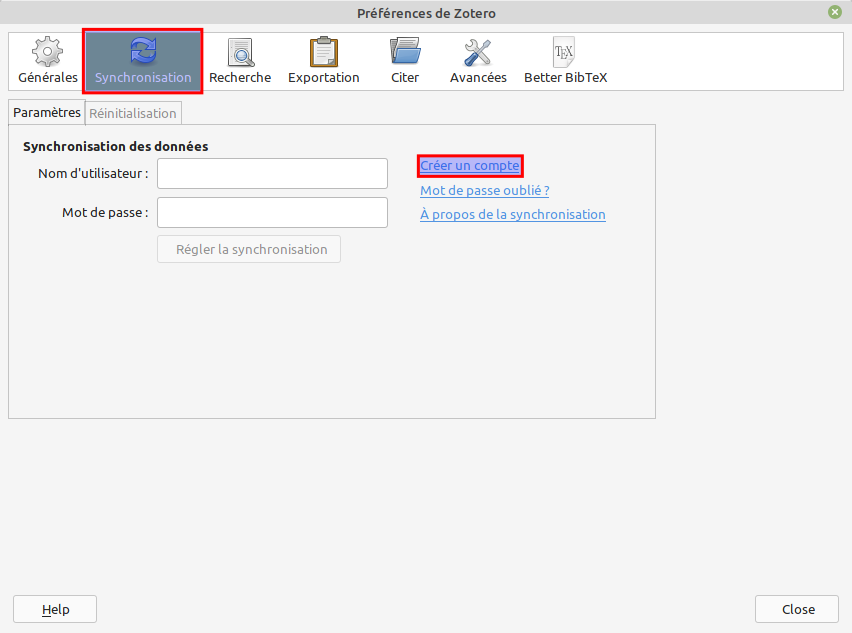
\includegraphics[width=12cm]{captures/zotero_01_compte}
					\caption{}
					\label{fig:zotero_01_compte}
				\end{figure}
			\end{center}
			\item Dans l'onglet Exportation \\
				Pour permettre le glisser-déposer de citations entre Zotero et TexStudio, choisir le format d'exportation \incmd{Better BibTeX Quick Copy}
				\begin{center}
					\begin{figure}[H]
						\centering
						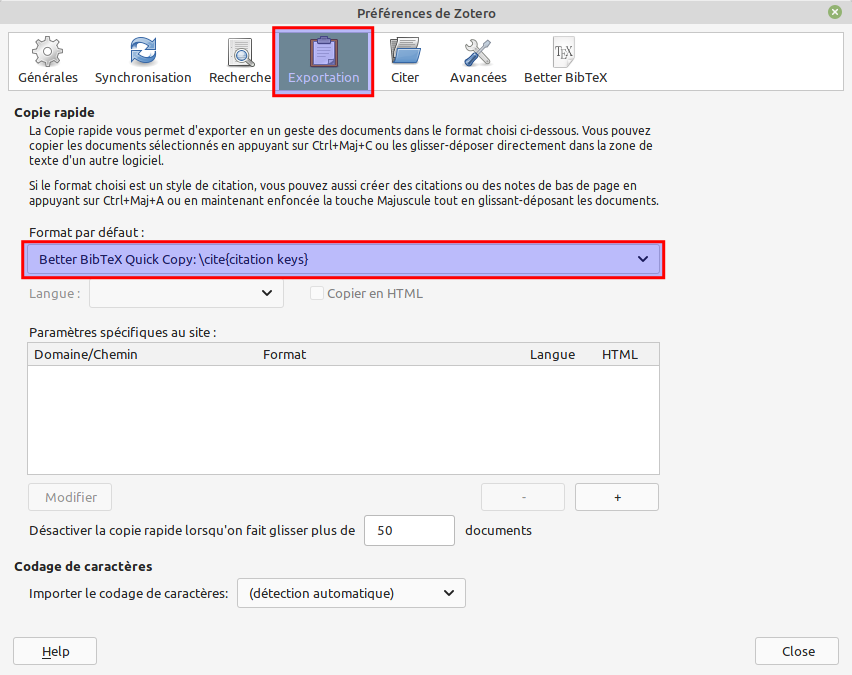
\includegraphics[width=12cm]{captures/zotero_02_exportation}
						\caption{}
						\label{fig:zotero_02_exportation}
					\end{figure}
				\end{center}
		\end{itemize}
	\item Configurer Better BibTeX.Tout se passe dans la boîte de dialogue 
			\begin{center}
				Édition \textrightarrow \ Préférences \ \textrightarrow \ Better BibTeX \textrightarrow Exportation \textrightarrow \ Copie rapide
			\end{center}
			Pour permettre le glisser-déposer de citations entre Zotero et TeXstudio, choisir le format citation LaTeX et taper autocite comme commande LaTeX.
			\begin{center}
				\begin{figure}[H]
					\centering
					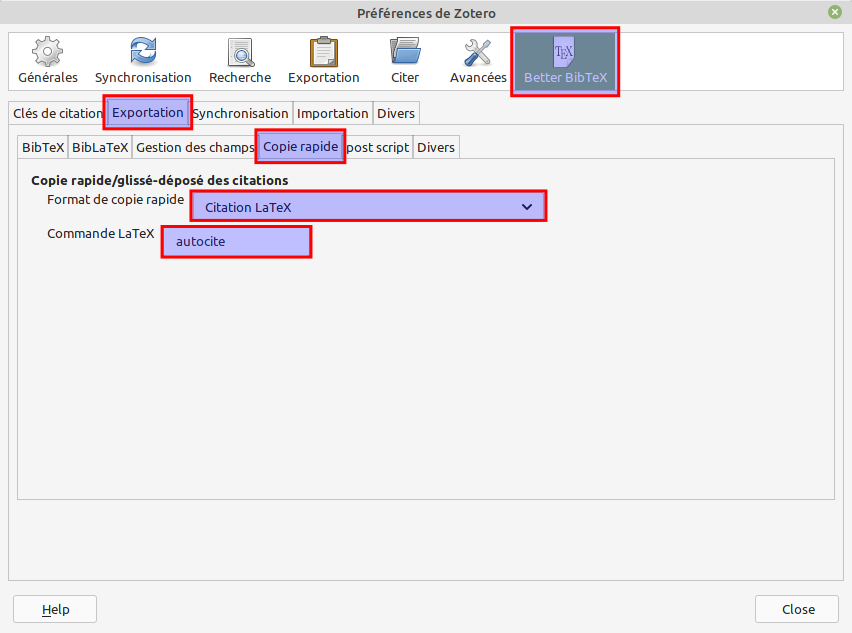
\includegraphics[width=12cm]{captures/zotero_03_better_bib_tex}
					\caption{}
					\label{fig:zotero_03_better_bib_tex}
				\end{figure}
			\end{center}
\end{enumerate}



\subsection{Configurer Texstudio}

Vérifiez que \incmd{biber} et le \incmd{Outil de bibliographie par défaut} (voir fig. \ref{fig:captureConfigBiber}).

\begin{center}
	\begin{figure}[H]
		\centering
		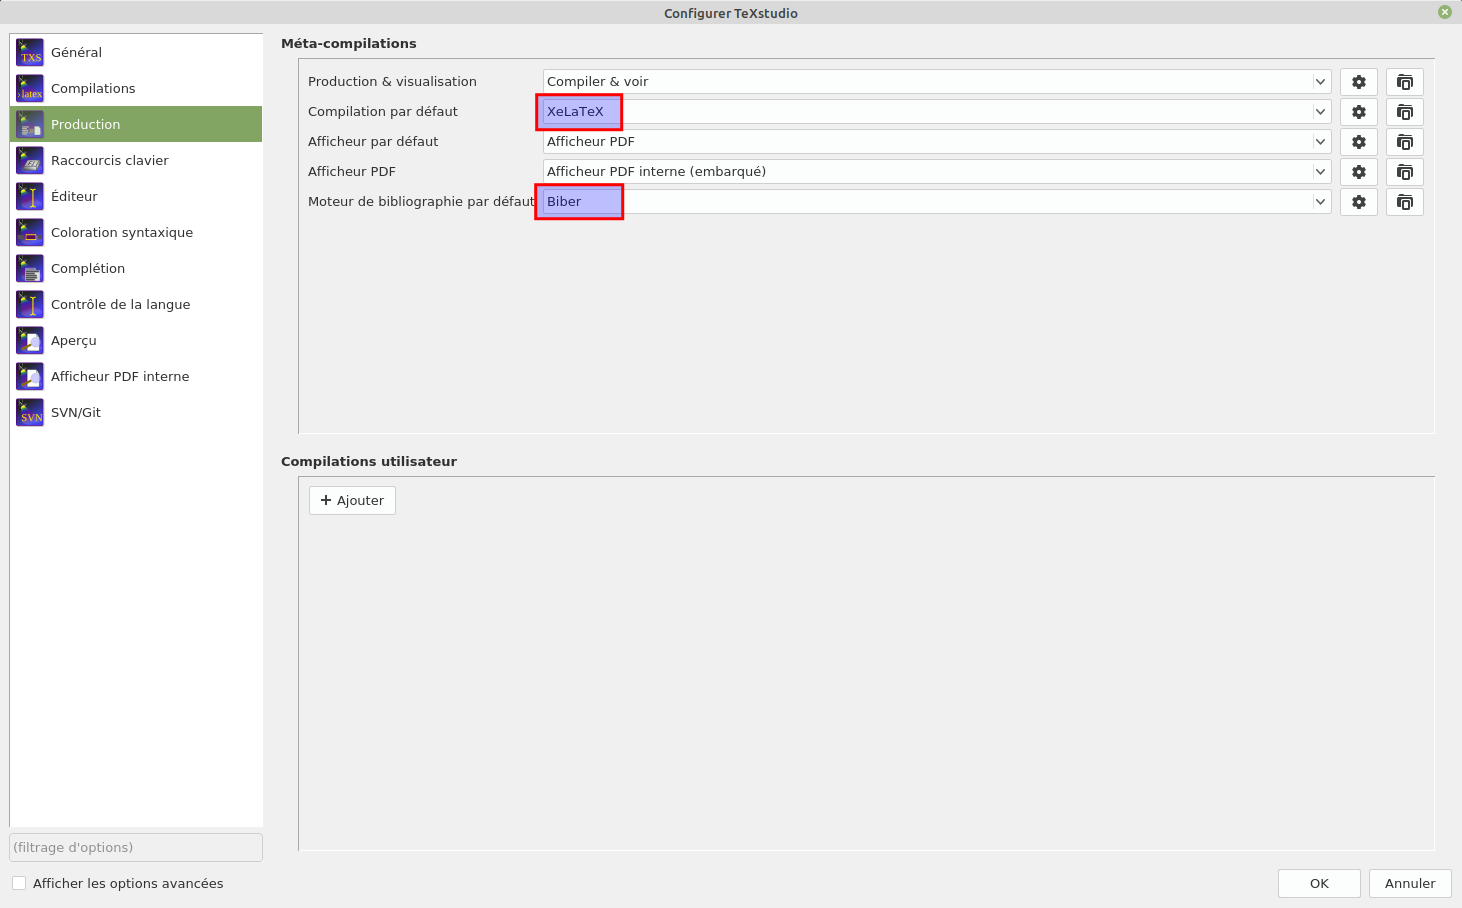
\includegraphics[width=12cm]{captures/Configurer_TeXstudio_production}
		\caption{}
		\label{fig:captureConfigBiber}
	\end{figure}
\end{center}

\nocite{CTANPackageBibLaTeX}
\printbibliography[heading=subbibliography, title=Liste des références]




\section{Index}

Pour générer un index :

\begin{enumerate}
	\item inclure un \mintinline{latex}{\makeindex} dans le préambule (ou le dé-commenter dans le template);
	\item déclarer les entrées d'index avec \mintinline{latex}{\index{entrée}};
	\item pour des sous-entrées : \mintinline{latex}{\index{Point(s)!confondus}}\mintinline{latex}{\index{Confondu(e)s!points}};
	\item placer un \mintinline{latex}{\printindex} à l'endroit où l'on veut faire afficher l'index.
\end{enumerate}

\remarque*{
	Si on veut faire des entrées d'index systématiquement pour toutes les définitions, on peut mettre \mintinline{latex}{\index} dans la définition de \mintinline{latex}{\emphdef} :
	\begin{center}
		\mintinline{latex}{\renewcommand{\emphdef}[1]{\emph{#1}\index{#1}}}.
	\end{center}
}




